\begin{figure}
    \centering
    \newcommand*{\subfigwidth}{0.49\textwidth}
    \begin{subfigure}[b]{\subfigwidth}
        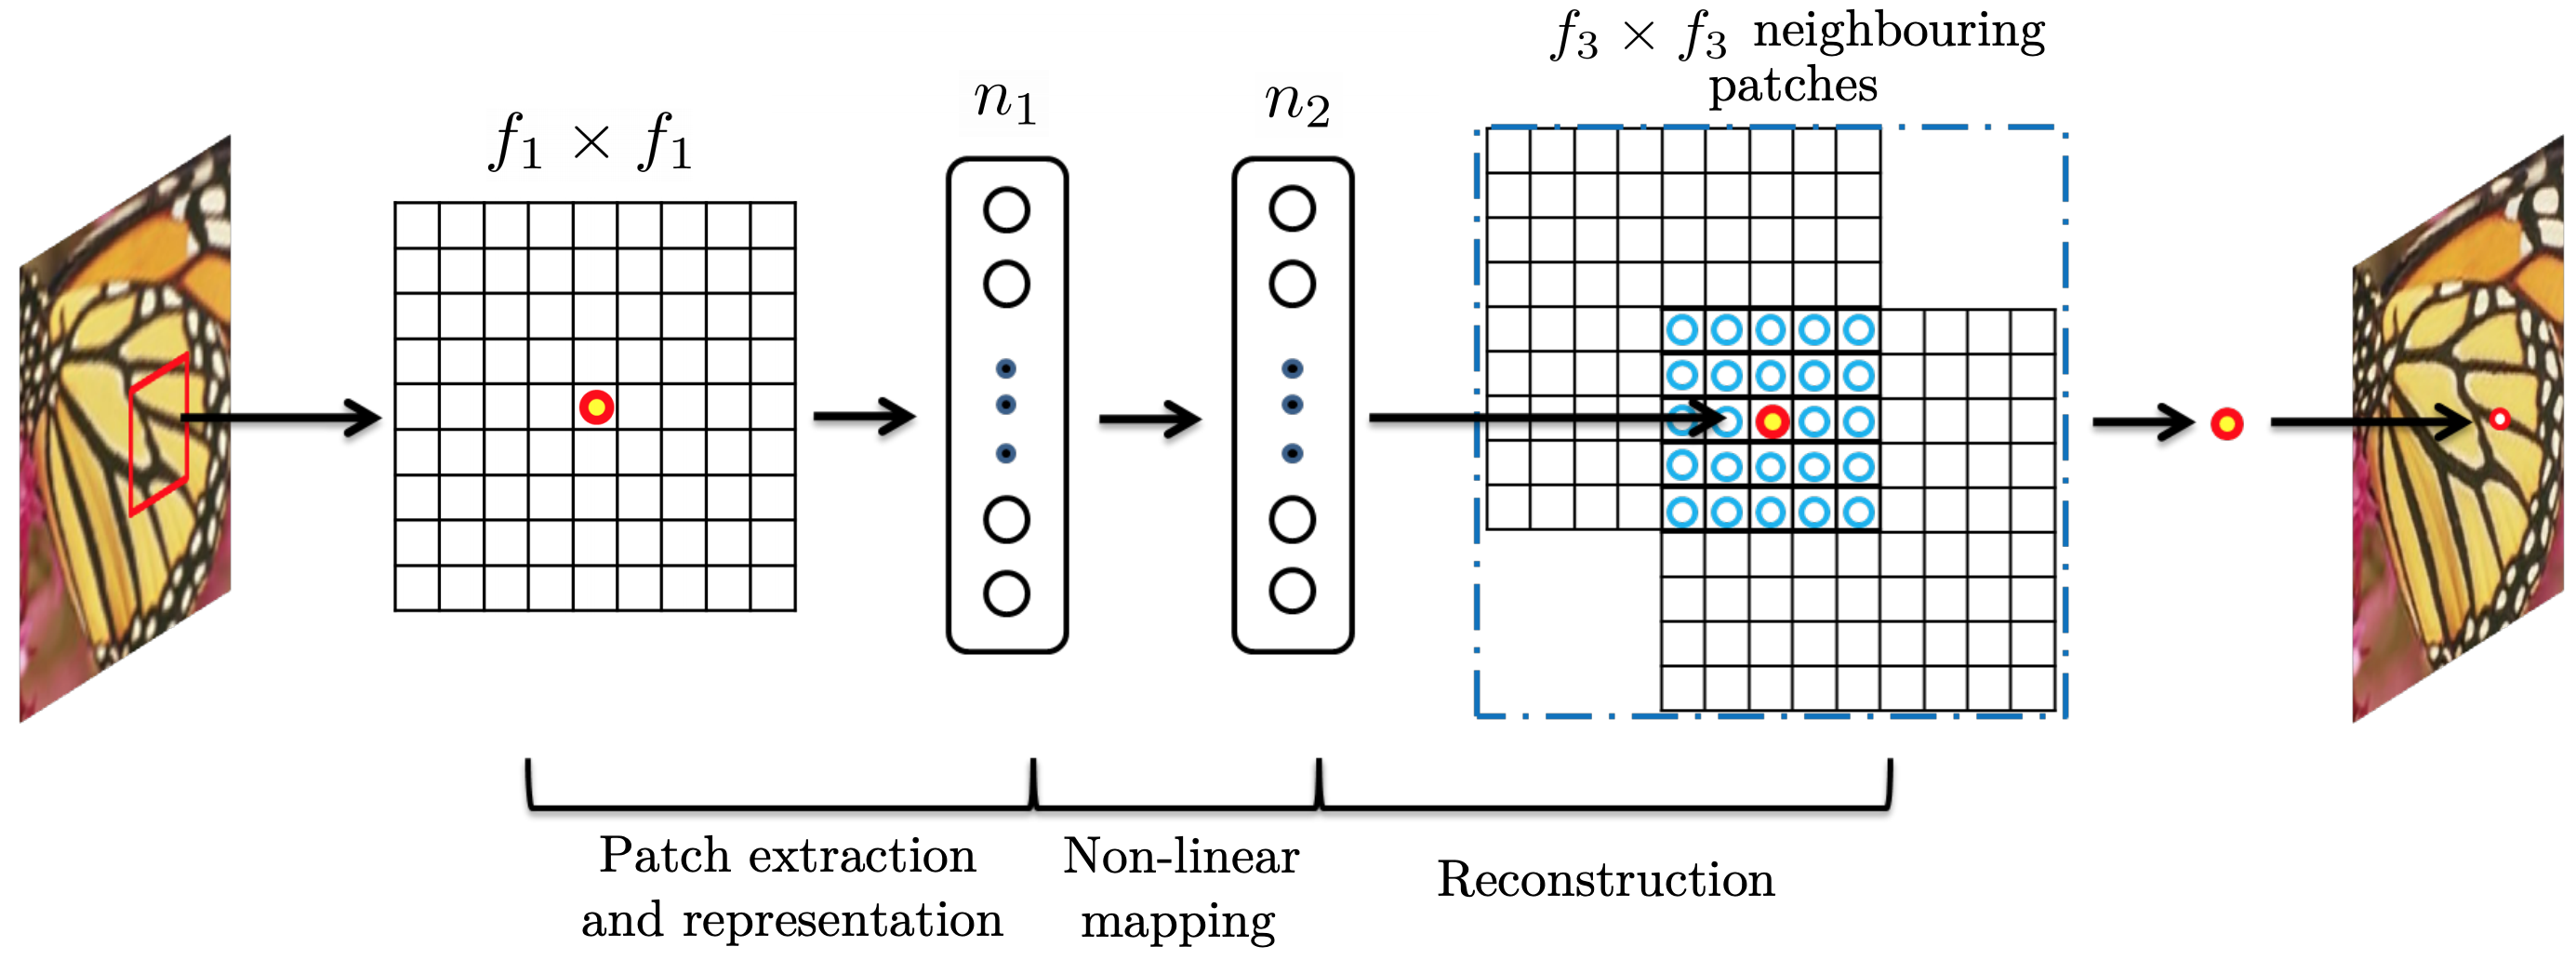
\includegraphics[width=\linewidth,keepaspectratio]{figures/neural_networks/sparse_coding.png}
        \caption{Sparse coding SR pipeline (see section~\ref{subsubsec:sparsecoding}).}\label{subfig:srcnnsparse}
    \end{subfigure}
    \vskip\baselineskip
    \begin{subfigure}[b]{\subfigwidth}
        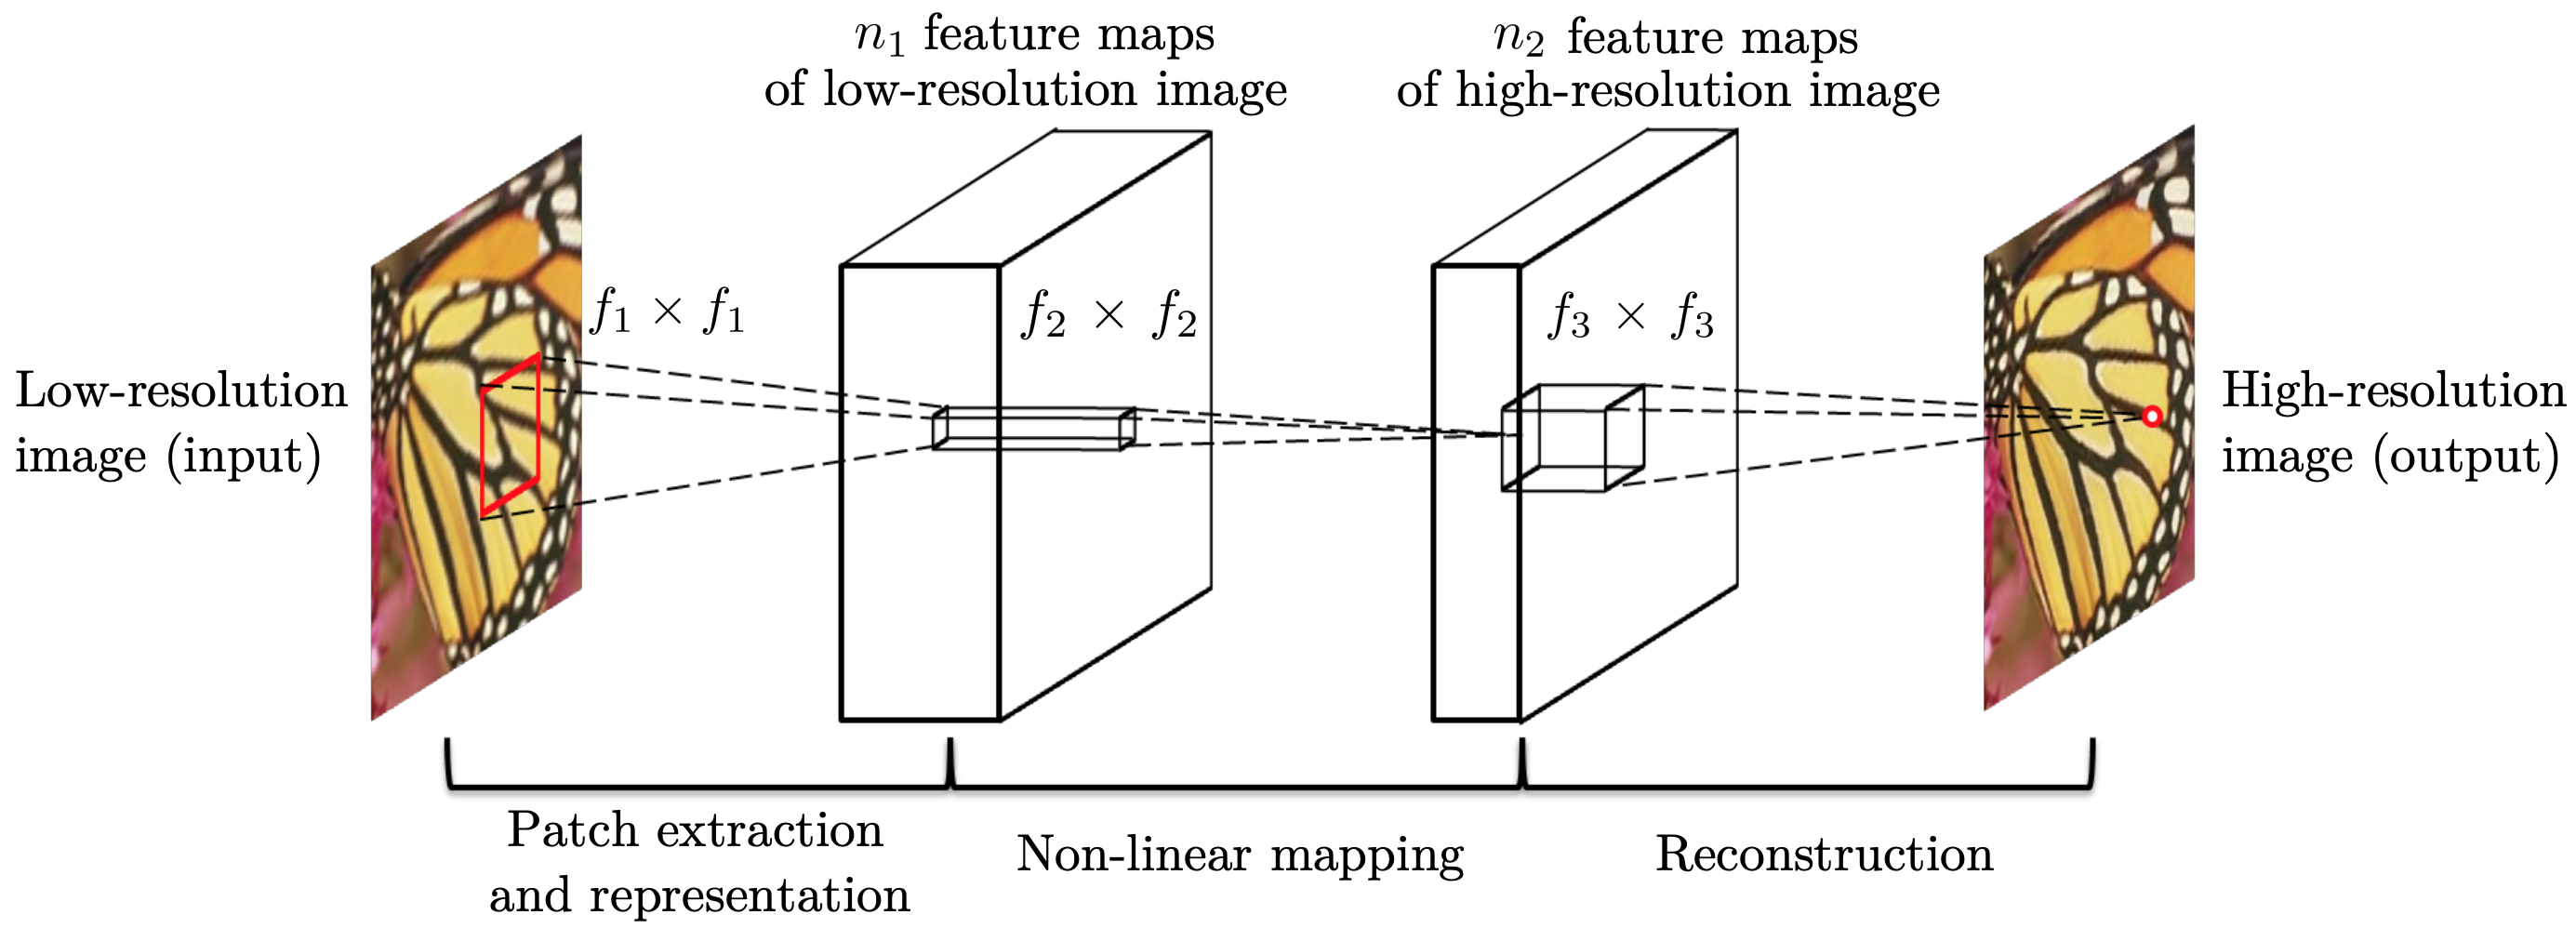
\includegraphics[width=\linewidth,keepaspectratio]{figures/neural_networks/srcnn.png}
        \caption{SRCNN pipeline.}\label{subfig:srcnn}
    \end{subfigure}
    \caption{Sparse coding SR and SRCNN comparison \cite{Dong_2016}. Note both pipelines operate on bicubic up-sampled images.}\label{fig:srcnn}
\end{figure}